% ==========================================================
% Template for Internship / Term Project Report
% Duration: 3 months | Length: 4 pages + References
% ==========================================================

\documentclass{article}
\usepackage{spconf,amsmath,graphicx,hyperref}

% -------------------------
% Additional useful packages
% -------------------------
\usepackage{booktabs}
\usepackage{siunitx}
\usepackage{enumitem}
\usepackage{stfloats}
\usepackage{tikz}
\usetikzlibrary{arrows.meta, positioning}

% -------------------------
% Custom definitions
% -------------------------
\def\x{{\mathbf x}}
\def\L{{\cal L}}

% -------------------------
% Title and Author Info
% -------------------------
\title{Your Project Title Goes Here}

\name{Your Name (Roll Number: XXXXX)}

\address{
Internship / Term Project Report\\
Trimester 7 / 8 / 9\\[0.5em]
B.Sc. (Honours) Data Science and Artificial Intelligence\\
Indian Institute of Technology Guwahati, India\\
\texttt{your-email@op.iitg.ac.in}
}


\begin{document}
\ninept
\maketitle

% \maketitle

% ==========================================================
% Abstract
% ==========================================================
\begin{abstract}
The abstract should provide a concise summary of the entire project.
It must clearly answer the following questions:
(1) What problem did you work on?
(2) Why is the problem important?
(3) What approach did you take?
(4) What were the key outcomes or insights?

\textbf{Good practice:}
\begin{itemize}[noitemsep]
    \item Write the abstract \emph{after} completing the report
    \item Keep it factual and precise (no storytelling here)
    \item Limit to 150--200 words
\end{itemize}

\emph{Example:}
This report presents the work carried out during a three-month internship on 
\emph{[problem domain]}. The objective was to \emph{[objective]}. A 
\emph{[method/approach]} was developed and evaluated using \emph{[data/tools]}. 
Experimental results indicate that \emph{[key outcome or insight]}.
\end{abstract}

% ==========================================================
% Keywords
% ==========================================================
\begin{keywords}
List 4--6 keywords that best describe your work (e.g., Machine Learning, Computer Vision, Optimization).
\end{keywords}

% ==========================================================
\section{Introduction}
% ==========================================================

The introduction sets the context for your work. Assume that the reader is 
technically trained but not familiar with your specific project.

\textbf{This section should:}
\begin{itemize}[noitemsep]
    \item Introduce the application or problem domain
    \item Explain why the problem matters (practical or research relevance)
    \item Briefly summarize what you did
\end{itemize}

\textbf{Good practice:}
\begin{itemize}[noitemsep]
    \item Avoid detailed technical explanations here
    \item Do not include results or conclusions
    \item End with a short paragraph describing the structure of the report
\end{itemize}

\emph{Example closing sentence:}
Section~2 describes the problem formulation and objectives. 
Section~3 details the methodology. 
Experimental results are presented in Section~4, followed by discussion and conclusions.

% ==========================================================
\section{Problem Statement and Objectives}
% ==========================================================

\subsection{Problem Statement}
Clearly and precisely define the problem you worked on.
A reader should be able to understand the problem without reading the rest of the report.

\textbf{Good practice:}
\begin{itemize}[noitemsep]
    \item Avoid vague statements such as ``we worked on AI''
    \item Specify constraints, assumptions, and scope
    \item Mention real-world relevance if applicable
\end{itemize}

\subsection{Objectives}
List the specific goals you aimed to achieve during the project.

\textbf{Good practice:}
\begin{itemize}[noitemsep]
    \item Objectives should be measurable or verifiable
    \item Use action verbs (design, analyze, evaluate, implement)
\end{itemize}

\emph{Example:}
\begin{enumerate}[noitemsep]
    \item To study existing approaches for \emph{[problem]}
    \item To design and implement a \emph{[model/system]}
    \item To evaluate performance using appropriate metrics
\end{enumerate}

% ==========================================================
\section{Methodology / Approach}
% ==========================================================

This section explains \emph{how} you addressed the problem.
It should be detailed enough for another student to reproduce your work.

\subsection{Overall Workflow}
Provide a high-level overview before diving into details.
You can include figures in your report for this (see Figure~\ref{fig:perceptron_convergence}).

\begin{figure}
    \centering
    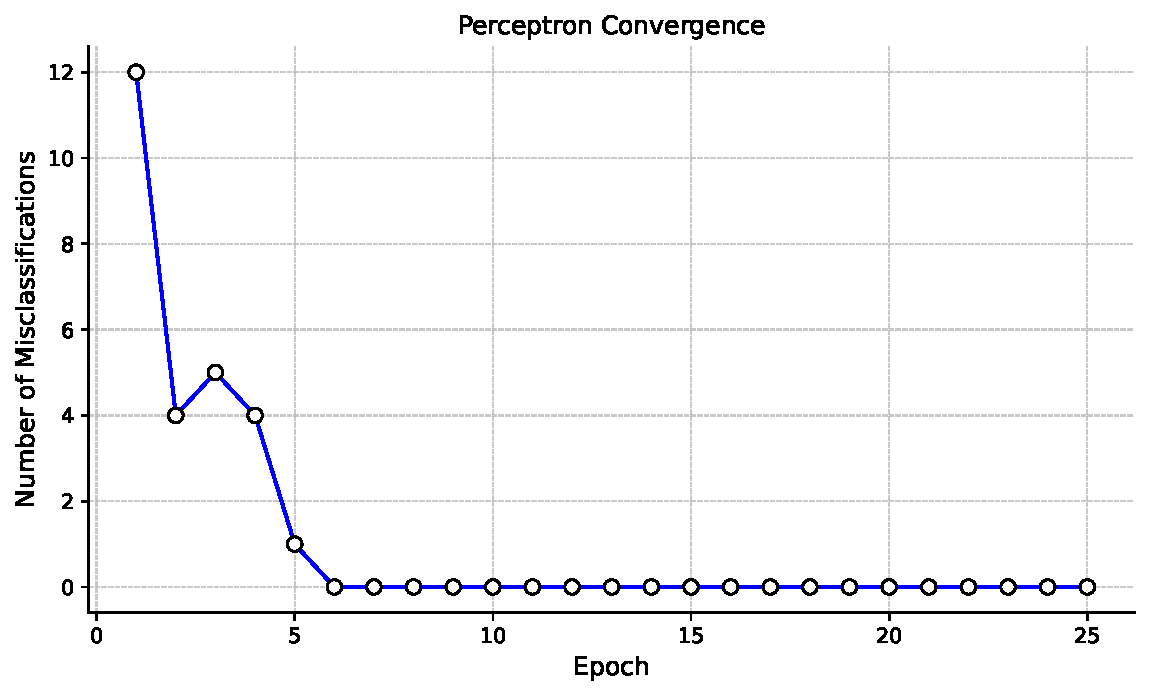
\includegraphics[height=5cm, width=9cm]{figures/perceptron_convergence.pdf}
    \caption{Illustration of perceptron convergence for a training set comprising of 100 sample points drawn from two classes (balanced).}
    \label{fig:perceptron_convergence}
\end{figure}
\textbf{Good practice:}
\begin{itemize}[noitemsep]
    \item Start from data or inputs and end with outputs
    \item Explain each block briefly in the text
\end{itemize}

% (TikZ figure remains unchanged)

\subsection{Technical Details}
Describe algorithms, models, tools, or frameworks used.

\textbf{Good practice:}
\begin{itemize}[noitemsep]
    \item Clearly justify design choices
    \item Reference prior work where applicable
    \item Include equations only when they add clarity
\end{itemize}

\emph{Example:}
The loss function used for training is given by
\begin{equation}
\L = \sum_{i=1}^{N} \ell(y_i, f(\x_i)),
\end{equation}
where $\ell(\cdot)$ denotes the task-specific loss.

% ==========================================================
\section{Experiments and Results}
% ==========================================================

This section presents the experimental setup and results objectively.

\subsection{Experimental Setup}
Describe datasets, tools, and evaluation protocols.

\textbf{Good practice:}
\begin{itemize}[noitemsep]
    \item Mention dataset size and splits
    \item Specify hardware and software environment
    \item Clearly define evaluation metrics
\end{itemize}

\subsection{Results}
Present results using tables and figures.

\textbf{Good practice:}
\begin{itemize}[noitemsep]
    \item Refer to every table and figure in the text
    \item Do not interpret results here (save that for Discussion)
\end{itemize}

% ==========================================================
\section{Discussion}
% ==========================================================

Interpret and analyze the results presented earlier.

\textbf{This section should address:}
\begin{itemize}[noitemsep]
    \item Why certain methods performed better or worse
    \item Trade-offs observed during experimentation
    \item Limitations of the approach
\end{itemize}

\textbf{Good practice:}
\begin{itemize}[noitemsep]
    \item Be honest about failures or challenges
    \item Connect observations back to objectives
\end{itemize}

% ==========================================================
\section{Conclusion and Future Work}
% ==========================================================

Summarize the work and reflect on learning outcomes.

\textbf{Good practice:}
\begin{itemize}[noitemsep]
    \item Do not repeat the abstract
    \item Highlight key contributions and insights
    \item Suggest realistic future improvements
\end{itemize}

\emph{Example future work:}
Future extensions could include exploring larger datasets, alternative models, or real-time deployment.

\textbf{Note to students:}  
Clear scientific writing is an essential research skill. Students are encouraged
to reflect on their learning process and presentation quality, and may consult
well-known resources on effective research writing and paper structure
(e.g., \cite{gopen1990science, knuth1984literate, peytonjones2003great}).

% ==========================================================
\section{Artifacts and Demonstrations}
% ==========================================================

This section provides links to external resources that complement the report.
Students are encouraged to share reproducible artifacts that demonstrate their
implementation, experiments, or system behavior.

\textbf{Examples of acceptable artifacts include:}
\begin{itemize}[noitemsep]
    \item Source code repositories (e.g., GitHub, GitLab)
    \item Technical blogs or project webpages
    \item Video demonstrations (e.g., YouTube, institutional cloud links)
    \item Interactive demos or dashboards (if applicable)
\end{itemize}

\textbf{Good practice:}
\begin{itemize}[noitemsep]
    \item Ensure links are publicly accessible or shared with appropriate permissions
    \item Clearly describe what each link contains
    \item Avoid linking raw folders without explanation
    \item Ensure content reflects your own work and contributions
\end{itemize}

\textbf{Example:}
\begin{itemize}[noitemsep]
    \item \textbf{Code Repository:} \url{https://github.com/username/project-name}
    \item \textbf{Project Blog:} \url{https://medium.com/@username/project-summary}
    \item \textbf{Video Demo:} \url{https://youtu.be/xxxxxx}
\end{itemize}

\textbf{Note:}
Use of AI-assisted tools (e.g., ChatGPT, Gemini, Copilot) is permitted to enhance
understanding and productivity. Students must ensure originality, proper attribution,
and a clear understanding of all submitted work.


% ==========================================================
% References
% ==========================================================
\vfill\pagebreak
{\fontsize{8}{9}\selectfont
\bibliographystyle{IEEEbib}
\bibliography{refs}
}

\end{document}

